\documentclass[11pt,letterpaper]{exam}
\RequirePackage{amssymb, amsfonts, amsmath, latexsym, verbatim, xspace, setspace, mathrsfs}
\usepackage{amsmath,amsthm,amssymb,amsfonts, 
hyperref, color, graphicx, enumitem}
\RequirePackage{tikz, pgflibraryplotmarks}
\usepackage{geometry}
\usepackage{graphicx}
\usetikzlibrary{calc}
\newcommand{\N}{\mathbb{N}}
\newcommand{\Z}{\mathbb{Z}}
\newcommand{\Q}{\mathbb{Q}}
 
\newenvironment{problem}[2][Problem:]{\begin{trivlist}
\item[\hskip \labelsep {\bfseries #1}\hskip \labelsep {\bfseries #2}]}{\end{trivlist}}

\newenvironment{claim}[2][Claim:]{\begin{trivlist}
\item[\hskip \labelsep {\bfseries #1}\hskip \labelsep {\bfseries #2}]}{\end{trivlist}}

\newenvironment{defn}[2][Definition:]{\begin{trivlist}
\item[\hskip \labelsep {\bfseries #1}\hskip \labelsep {\bfseries #2}]}{\end{trivlist}}

% Here's where you edit the Class, Exam, Date, etc.
\newcommand{\class}{Sec 4}
\newcommand{\term}{Winter 2019}
\newcommand{\examnum}{}
\newcommand{\examdate}{Quiz 7}
\newcommand{\timelimit}{}

% For an exam, single spacing is most appropriate
\singlespacing
% \onehalfspacing
% \doublespacing

% For an exam, we generally want to turn off paragraph indentation
\parindent 0ex

\begin{document} 

% These commands set up the running header on the top of the exam pages
\pagestyle{head}
\firstpageheader{ \Large{Name:}}{\Large{Quiz 7}}{}
\runningheader{\class}{\examnum\ - Page \thepage\ of \numpages}{\examdate}
\runningheadrule

%\begin{flushright}
%\begin{tabular}{p{2.8in} r l}
%\textbf{\class} & \textbf{Name:} & \makebox[2in]{\hrulefill}\\
%\textbf{\term} &&\textbf{\examnum}\\
%\textbf{\examdate} &&
%\textbf{Time Limit:  \timelimit}  \\ 
%\end{tabular}\\
%\end{flushright}
%\rule[1ex]{\textwidth}{.1pt}




%\begin{minipage}[t]{3.7in}
%\vspace{0pt}
%\begin{itemize}

%% \item \textbf{DO NOT open the exam booklet until you are told to begin. You should write your name and section number at the top and read the instructions.}

%% \vfill

%% \item Organize your work, in a reasonably neat and coherent way, in
%% the space provided. If you wish for something to not be graded, please strike it out neatly. I will grade only work on the exam paper, unless you clearly indicate your desire for me to grade work on additional pages.

%% \item You may use any results from class, homework or the text, but you must cite the result you are using. You must prove everything else.

%% \item You needn't spend your time rewriting definitions or axioms on the exam.

%% \end{itemize}


%% \end{minipage}
%% \hfill
%% \begin{minipage}[t]{2.3in}
%% \vspace{0pt}
%% %\cellwidth{3em}
%% \gradetablestretch{2}
%% %Uncomment this line to make the table display 100 as the total no matter what. This is good for tests with an ommit question.
%% %\settabletotalpoints{100}
%% \vqword{Problem}
%% \addpoints % required here by exam.cls, even though questions haven't started yet.	
%% \gradetable[v]%[pages]  % Use [pages] to have grading table by page instead of question

%% \end{minipage}

%% \begin{itemize}


%% \item You may use the text, my class notes and/or any notes and study guides you have created. You may use a calculator. You may not use a cell phone or computer.


%% \item When you have completed your test, hand it to me and go have a great weekend!

%% \item There is a single bonus problem at the end of the test. It would be best to work first on the main test as this problem is only worth 5 points and will be graded strictly.

%% \end{itemize}

%%\newpage

\begin{questions}
\addpoints
\question 
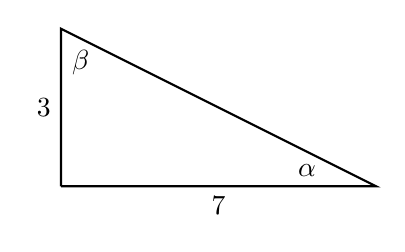
\begin{tikzpicture}[thick]
  \draw(0,0) -- (90:2cm) node[midway,left]{$3$} -- (0:4cm) node[midway,above right]{} -- (0,0) node[midway,below]{$7$};
  
\draw (4,0) -- ++(180:0.8cm)  node at ($(167:0.9cm)+(4,0)$) {$\alpha$} -- cycle;
\draw[] (0,2) -- ++(-90:0.8cm) node at ($(-60:0.5cm)+(0,2)$) {$\beta$} -- cycle;
\end{tikzpicture}

for the right angle triangle above, calculate

\begin{parts}
  \part[2] $\sin\alpha$
  \part[2] $\sin\beta$
  \part[2] $\cos\beta$
  \part[2] $\cos\beta + \sin\alpha$
  \part[2] $\tan\alpha$
\end{parts}

    

%% \question F
%% \begin{parts}
%% \part[5] $\displaystyle \frac{(2\cdot x^{-3}\cdot y^7)^2}{(4\cdot x^{-4}\cdot y^3)}$
%% \vfill
%% \part[5] $\displaystyle \frac{2a^3b^4+8b^2}{4a^2b}\div (5a^{-1}b^3)$
%% \vfill
%% \end{parts}


%% \newpage 
%% \addpoints

%% \question Factor the following expressions.
%% \begin{parts}
%%   \part[3] $x^2 - 2 x -24$
%%   \vfill
%%   \part[3] $4x^3 - 12x^2 + 8x$
%%   \vfill
%% \end{parts}

%% \question[4] What are the roots the polynomials in the previous question.
%% \vfill
%\bonusquestion[5] This is a bonus question. It has points but they are not added on the cover page.
%\vfill

\end{questions}
\end{document}
